\section{Metrics Used For Evaluation}

To evaluate the performance of the autoencoder, the anomaly detection procedure and the CNN-model, several metrics are used. 

\subsection{Autoencoder}

To evaluate how well the autoencoder is able to reconstruct the input data,  Mean Squared Error (MSE), Peak Signal-To-Noise Ratio (PSNR), Structural Similarity Index Measure (SSIM) and a threshold image sum method are used. 
\par
MSE takes the avarage of the squared differences between each pixel in the original image and the reconstructed image. PSNR is a metric that express the ratio between the maximum value of each pixel and the MSE. SSIM is a more complex method that considers changes in the structural nature of the images. 
\par
The threshold image sum method is a method that first creates a mask of the difference of both images to highlight areas where the difference is significant. The total sum of the mask is then calculated and used as a metric. The idea for this method is to take advantage of the fact that anomalous images should have big differences in specific areas of the original image and reconstructed image.

\subsection{Anomaly detection procedure}

The metrics uses for evaluating our anomaly detection procedure are Reciver Operator Characteristic Area Under the Curve (ROC-AUC), Accuracy and F1-score. ROC-AUC is a metric that evaluates the performance of the model by calculating the area under the curve of the ROC-curve. The ROC-curve is a curve that shows the true positive rate against the false positive rate. Accuracy is a metric that calculates the ratio between the number of correct predictions and the total number of predictions. F1-score is a metric that calculates the mean of precision and recall.

\subsection{CNN-model}
For evaluating the CNN model's performance in classifying bottle images, we use several standard classification metrics, such as: accuracy, precision, recall, and F1-score.
Accuracy measures the overall correct predictions ratio, while precision indicates the model's ability to identify true positives correctly. 
Recall shows how well the model identifies all relevant cases, and F1-score provides a balanced measure between precision and recall. Additionally, we use a confusion matrix to visualize the model's performance across all classes, showing how well the model distinguishes between different types of bottles and defects.

\begin{figure}[H]
    \centering
    \begin{minipage}{0.48\textwidth}
        \centering
        \includegraphics[scale=0.25]{src/images/heatmap_metric.png}
        \vspace{-0.3cm}
        \caption{Confusion matrix heatmap}
        \label{fig:heatmap}
    \end{minipage}
    \hfill
    \begin{minipage}{0.48\textwidth}
        \centering
        \vspace{0.4cm}
        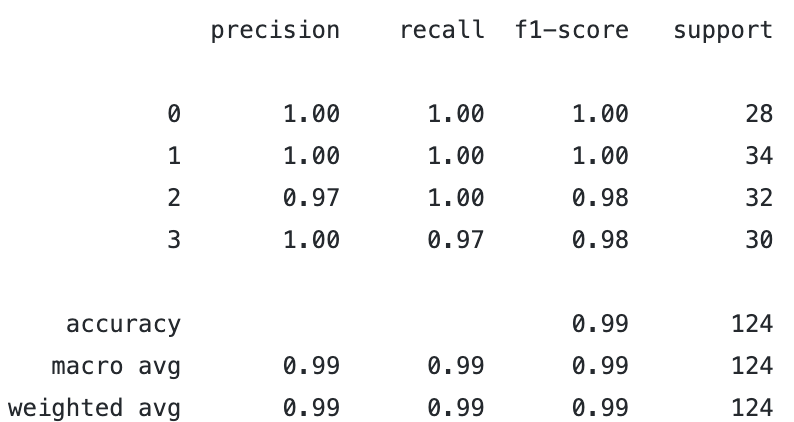
\includegraphics[scale=0.33]{src/images/cnn_report.png}
        \vspace{0.2cm}
        \caption{Classification report}
        \label{fig:report}
    \end{minipage}
\end{figure}


\subsection{Calculating the metrics}

Formulas for some of the metrics are defined as follows:

\begin{align*}
    \text{MSE} &= \frac{1}{n} \sum_{i=1}^{n} (x_i - \hat{x}_i)^2 \\
    \text{PSNR} &= 20 \cdot \log_{10} \left( \frac{\text{MAX\_VAL}}{\sqrt{\text{MSE}}} \right) \\
    \text{SSIM} &= \frac{(2\mu_x\mu_y + c_1)(2\sigma_{xy} + c_2)}{(\mu_x^2 + \mu_y^2 + c_1)(\sigma_x^2 + \sigma_y^2 + c_2)} \\
    F_1 &= \frac{2TP}{2TP + FP + FN} \\
    \text{Accuracy} &= \frac{\text{Correct Predictions}}{\text{Total number of images}} \\
\end{align*}

Thresholded images (masks) are created by applying a threshold function to each pixel of the image. The threshold function is defined as:

\begin{align*}
    f(x) &= 
    \begin{cases}
        \text{max\_val}(x) & \text{if } x > \text{threshold} \\
        0 & \text{otherwise}
    \end{cases} 
\end{align*}

and to calculate the sum of the mask, the values for each pixel and each channel are summed up.
\par
The ROC-AUC metric is best illustrated with a figure:
\begin{figure}[H] 
    \centering
    \begin{tikzpicture}
        \begin{axis}[
            width=10cm, height=8cm,
            xlabel={False Positive Rate (FPR)},
            ylabel={True Positive Rate (TPR)},
            xmin=0, xmax=1,
            ymin=0, ymax=1,
            grid=both,
            grid style={dashed, gray!30},
            legend pos=south east,
            legend style={font=\small},
            axis lines=left,
            axis line style={-},
            samples=100
        ]
        % Random classifier line (diagonal)
        \addplot [dashed, gray] coordinates {(0,0) (1,1)};
        \addlegendentry{Random Classifier}

        % Example ROC curve
        \addplot [
            name path=f,
            thick,
            smooth,
            blue,
        ] coordinates {
            (0.0, 0.0)
            (0.1, 0.6)
            (0.2, 0.75)
            (0.4, 0.85)
            (0.6, 0.9)
            (0.8, 0.95)
            (1.0, 1.0)
        };
        \addlegendentry{Anomaly Detection Procedure}

        \addplot [
            name path=g,
            draw=none
        ] coordinates {
            (0,0)
            (1,0)
        };
        \addplot[
            blue!20, opacity=0.5
            ] fill between[of=f and g, soft clip={domain=-2:2}];

        \end{axis}
    \end{tikzpicture}
    \caption{ROC-AUC visualized as the area under the ROC-curve.}
    \label{fig:ROCAUC}
\end{figure}